\documentclass{ximera}


\title{Central projection in SG}

\begin{document}
\begin{abstract}
In this activity, we venture deeper into our exploration of spherical
geometry under central projection.
\end{abstract}
\maketitle

\subsection*{Central projection preserves lines}

We all probably realize that you can't make a perfect map of the world; that
is, you can't make a map so that angles on the map are equal to the
corresponding angles on the sphere and straight lines on the map correspond to
great circular arcs on the sphere. We do the next best thing--we make two maps
of the sphere, one that has the property that angles are faithfully
represented and the other for which straight lines on the map correspond to
shortest paths on the sphere. We start with a simple way to make a map for
which straight lines on the map correspond to shortest paths on the sphere.
The map coordinates we use to do this are the \textit{central projection
coordinates} we learned about previously.%in Part \ref{III}.

Now \textbf{SG} is a $K$-geometry %in the sense of Part \ref{III} 
since, in
$\left(  x,y,z\right)  $-coordinates, the equation for the $R$-sphere becomes%
\[
K\left(  x^{2}+y^{2}\right)  +z^{2}=1
\]
with%
\[
K=\frac{1}{R^{2}}%
\]
and the Euclidean dot product is given by the $K$-dot product. So all
the computations of $K$-geometry hold for Spherical Geometry as long
as we understand that we are computing it in $\left( x,y,z\right)
$-coordinates.

\begin{exercise}
Show that central projection of a point on the $R$-sphere in $\left(  \hat
{x},\hat{y},\hat{z}\right)  $-space to the plane $\hat{z}=R$ is the same as
central projection of the corresponding point in $\left(  x,y,z\right)
$-coordinates to the plane $z=1$.

Hint: Recall that in central projection

\begin{tabular}
[c]{cc}%
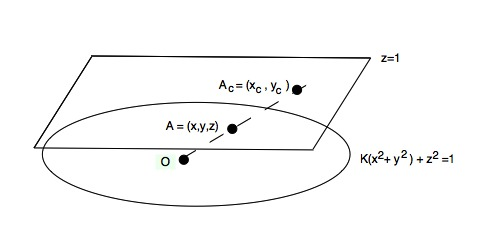
\includegraphics{MXAJBZ0K.jpg}%
 &
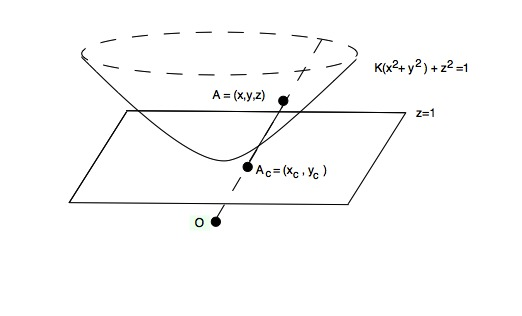
\includegraphics{MXAJBZ0L.jpg}%
\end{tabular}
So,%
\begin{equation}
r\cdot\left( x_{c},y_{c},1\right) =\left( x,y,z\right).
\end{equation}
and write the corresponding relation $\hat{r}\left(
\hat{x}_{c},\hat{y}_{c},R\right) =\left( \hat{x},\hat
    {y},\hat{z}\right) $ in $\left( \hat{x},\hat{y},\hat{z}\right)
    $-coordinates. Conclude that $\hat{r}=r$. (Why?)
\end{exercise}

\begin{exercise}
Show that lines (i.e. shortest paths in \textbf{SG}) correspond
under central projection to straight lines in the $\left(  x_{c},y_{c}\right)
$-coordinates.

Hint: See Exercise 13.2 %ref{73}
a). Or just write the equation for a line in
$\left(  x_{c},y_{c}\right)  $-coordinates and substitute 
\begin{align*}
x_{c}  &=\frac{x}{z}\\
y_{c}  &=\frac{y}{z}.
\end{align*}
Then reverse the process.
\end{exercise}

\subsection*{Spherical area computed in central projection coordinates}

Recall that %in Part \ref{III} 
we learned how to compute the $K$-area in
$K$-geometry of a region $G$ given by a region $G_{c}$ in the $\left(
x_{c},y_{c}\right)  $-plane. That is, we learned how to compute the area of a
region $\hat{G}$ on the $R$-sphere given by a region $G_{c}$ in the $\left(
x_{c},y_{c}\right)  $-plane via
\[
\int\nolimits_{G_{c}}
\sqrt{\left\vert
\begin{array}
[c]{cc}%
\frac{dX}{dx_{c}}\bullet_{K}\frac{dX}{dx_{c}} & \frac{dX}{dy_{c}}\bullet
_{K}\frac{dX}{dx_{c}}\\
\frac{dX}{dx_{c}}\bullet_{K}\frac{dX}{dy_{c}} & \frac{dX}{dy_{c}}\bullet
_{K}\frac{dX}{dy_{c}}%
\end{array}
\right\vert }dx_{c}dy_{c}.
\]

\begin{exercise}
Show that, if a region $\hat{G}$ on the $R$-sphere is
parametrized by a region $G_{c}$ in $\left(  x_{c},y_{c}\right)
$-coordinates, then the area $\hat{A}$ of $\hat{G}$ is given by the formula%
\[
\hat{A}=%
%TCIMACRO{\dint \nolimits_{G_{c}}}%
%BeginExpansion
{\displaystyle\int\nolimits_{G_{c}}}
%EndExpansion
\left(  K\left(  x_{c}^{2}+y_{c}^{2}\right)  +1\right)  ^{-3/2}dx_{c}dy_{c}.
\]

\end{exercise}


\end{document}



